\documentclass[11pt]{article}
\usepackage[margin=1in]{geometry}
\usepackage{graphicx}
\usepackage{amsmath}
\usepackage{amssymb}
\usepackage{float}
\usepackage{subcaption}

\title{June 24, 2021 Meeting Agenda}

\begin{document}
\maketitle

\section{Joint estimation of $\mu_p$ and $\mu_t$, Ad-hoc algorithm}
  \subsection{Key Points}
    \begin{itemize}
      \item The ad-hoc algorithm appears to be insensitive to initial parameters. I varied the initial values of both $\mu_p$ and $\mu_t$, regardless of the initial values, it converged to $\mu_p=13.2$ and $\mu_t=0.065$.
      \item Including all judges in our estimation of $\mu_t$ reduced our estimate of $\mu_t$ from 0.08 to 0.065. Table \ref{tab:my-table} shows how the values of $\mu_p$ and $\mu_t$ evolve during the algorithm.
      \item I redid the Negative log likelihood vs $\mu_p$ plot, plotting both the optimal value of $\mu_p$ we get using brute force, and the value we get from the optimizer. The plots are in Figure \ref{fig-nll}.

    \end{itemize}


    \begin{figure}[H]
      \centering
        \begin{subfigure}[b]{0.45\textwidth}
          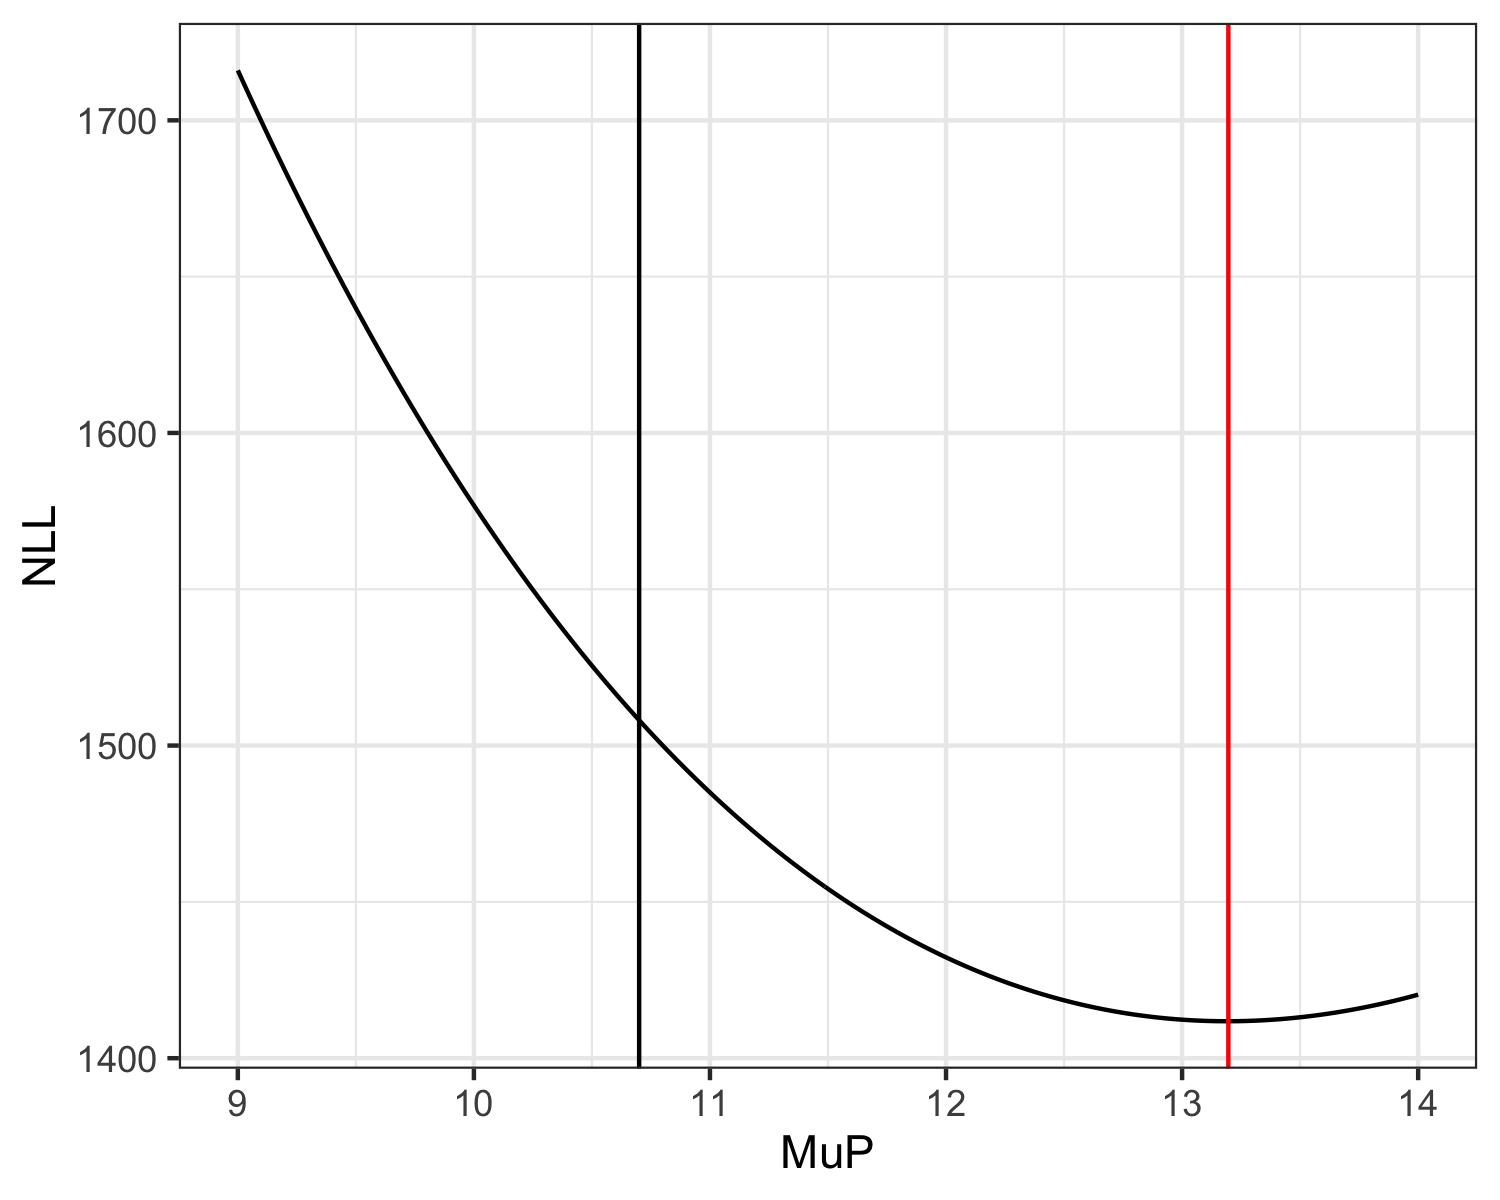
\includegraphics[width=\textwidth]{../../../output/figures/Optimization/opt_data_1.png}
          \caption{Initial Value}
          \label{fig:f1}
        \end{subfigure}
        \hfill
        \begin{subfigure}[b]{0.45\textwidth}
          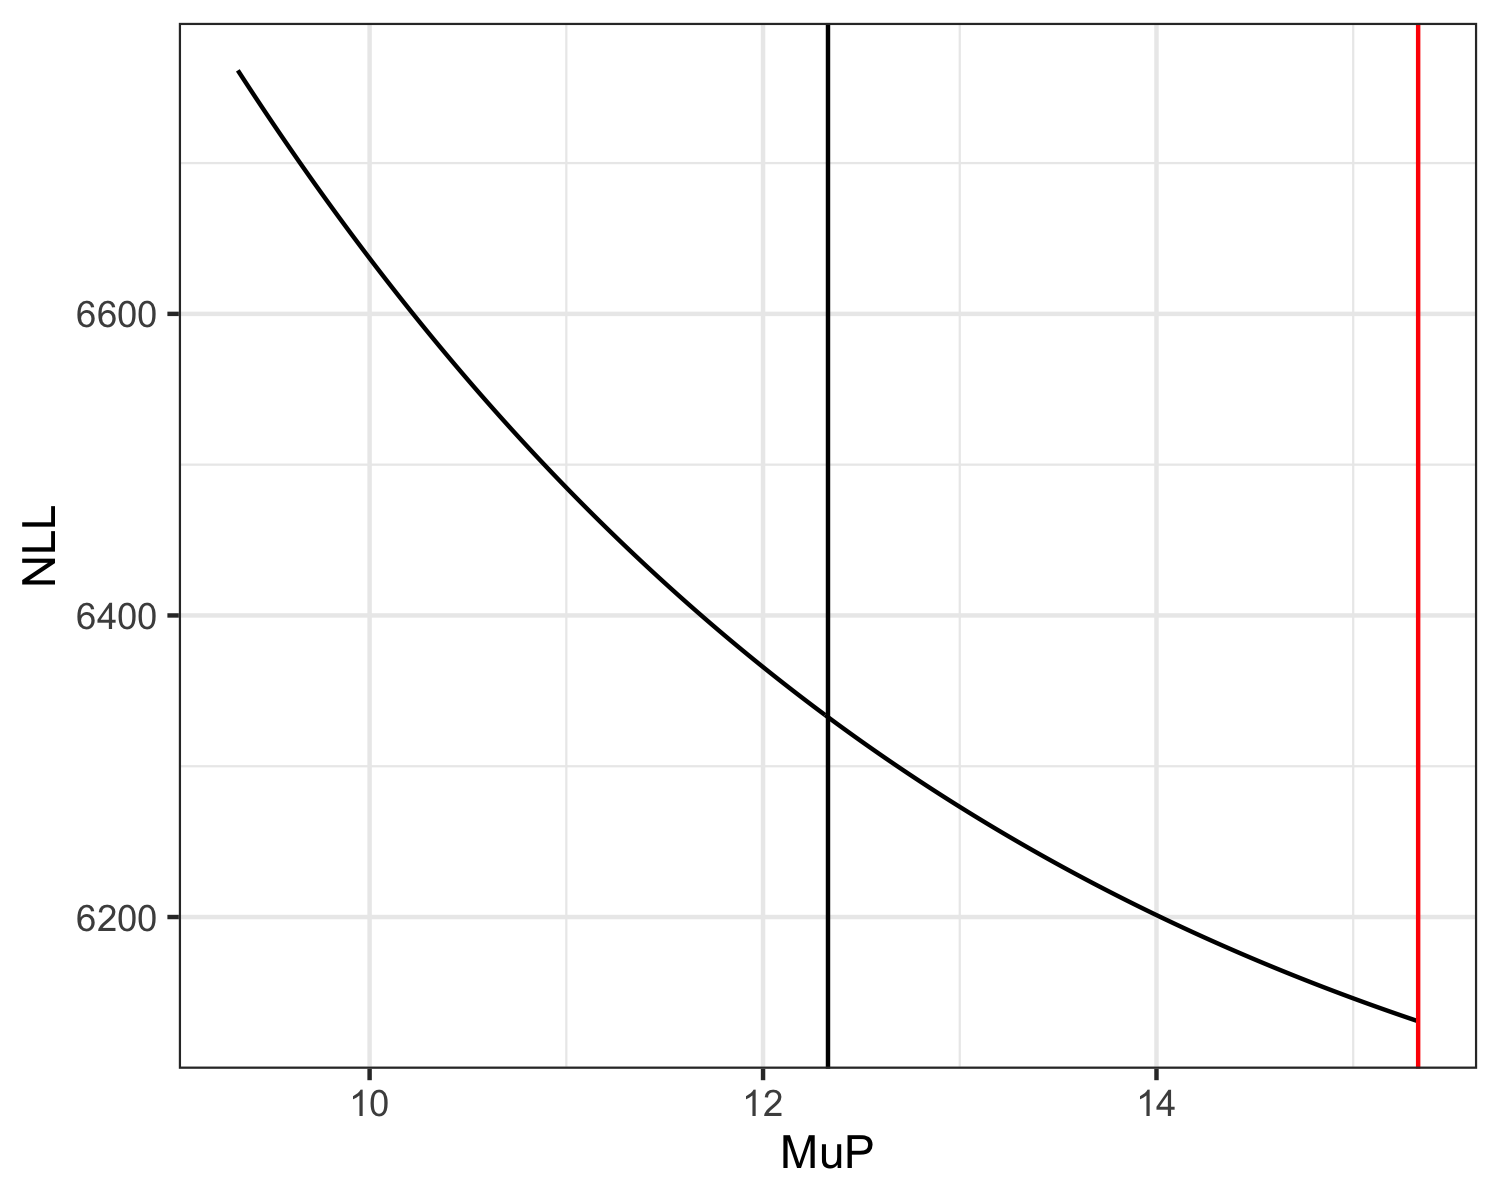
\includegraphics[width=\textwidth]{../../../output/figures/Optimization/opt_data_2.png}
          \caption{Iteration 1}

        \end{subfigure}
        %\hfill
        \begin{subfigure}[b]{0.45\textwidth}

          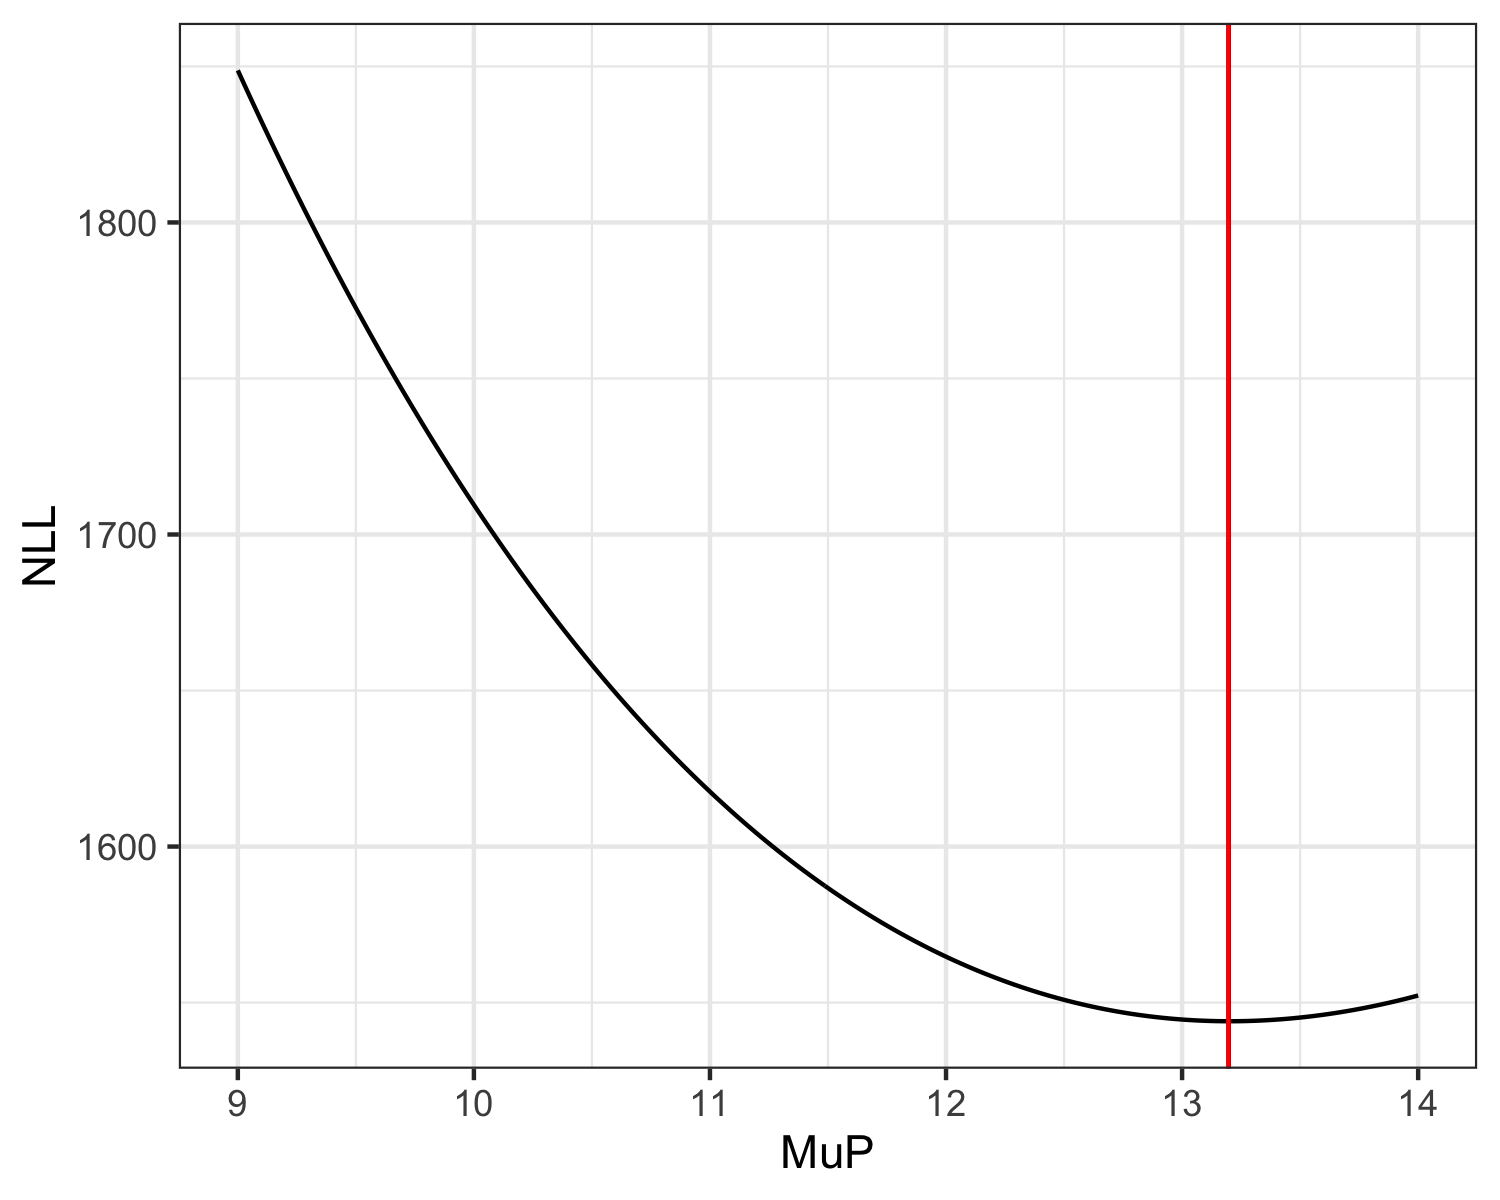
\includegraphics[width=\textwidth]{../../../output/figures/Optimization/opt_data_3.png}
          \caption{Iteration 2}

        \end{subfigure}
        \caption{Negative log likelihood vs $\mu_p$, the brute force optimizer is the red line}
        \label{fig-nll}
    \end{figure}

    \begin{table}[H]
    \centering
      \caption{Evolution of $\mu_p$ and $\mu_t$}
      \label{tab:my-table}
      \begin{tabular}{|l|l|l|}
      \hline
      \textbf{MuP} & \textbf{MuT} & \textbf{Iteration} \\ \hline
      10.700       & 0.140        & 0                  \\ \hline
      12.988       & 0.066        & 1                  \\ \hline
      13.197       & 0.065        & 2                  \\ \hline
      13.201       & 0.065        & 3                  \\ \hline
      \end{tabular}
    \end{table}

\section{Gaussian EM Algorithm}
  \subsection{Key Points}
    \begin{itemize}
      \item I plotted the mean value of $X_1^i,X_2^i,D_1^i,D_2^i$ in each iteration of the EM algorithm, the figure is below.
    \end{itemize}

    \begin{figure}[H]
      \centering
        \begin{subfigure}[b]{0.45\textwidth}
          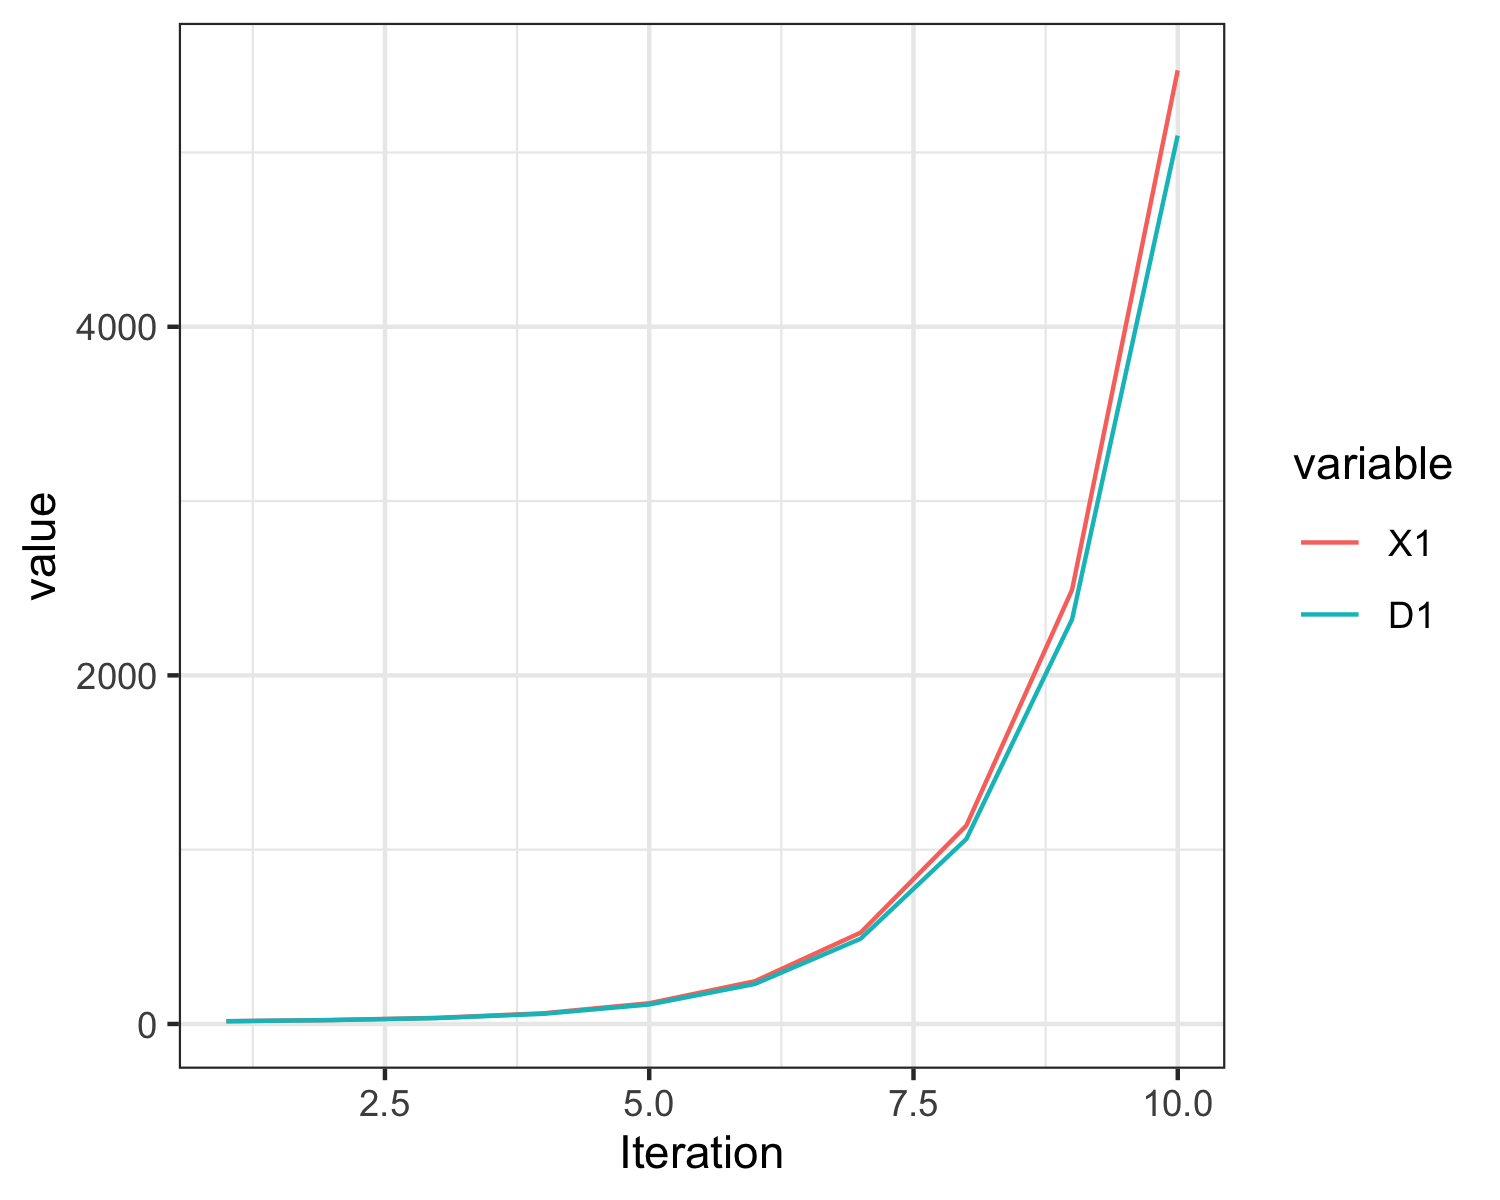
\includegraphics[width=\textwidth]{../../../output/figures/Optimization/x1_plot.png}
          \caption{Mean value of $X_1^i,D_1^i$}
          \label{fig:f1}
        \end{subfigure}
        \hfill
        \begin{subfigure}[b]{0.45\textwidth}
          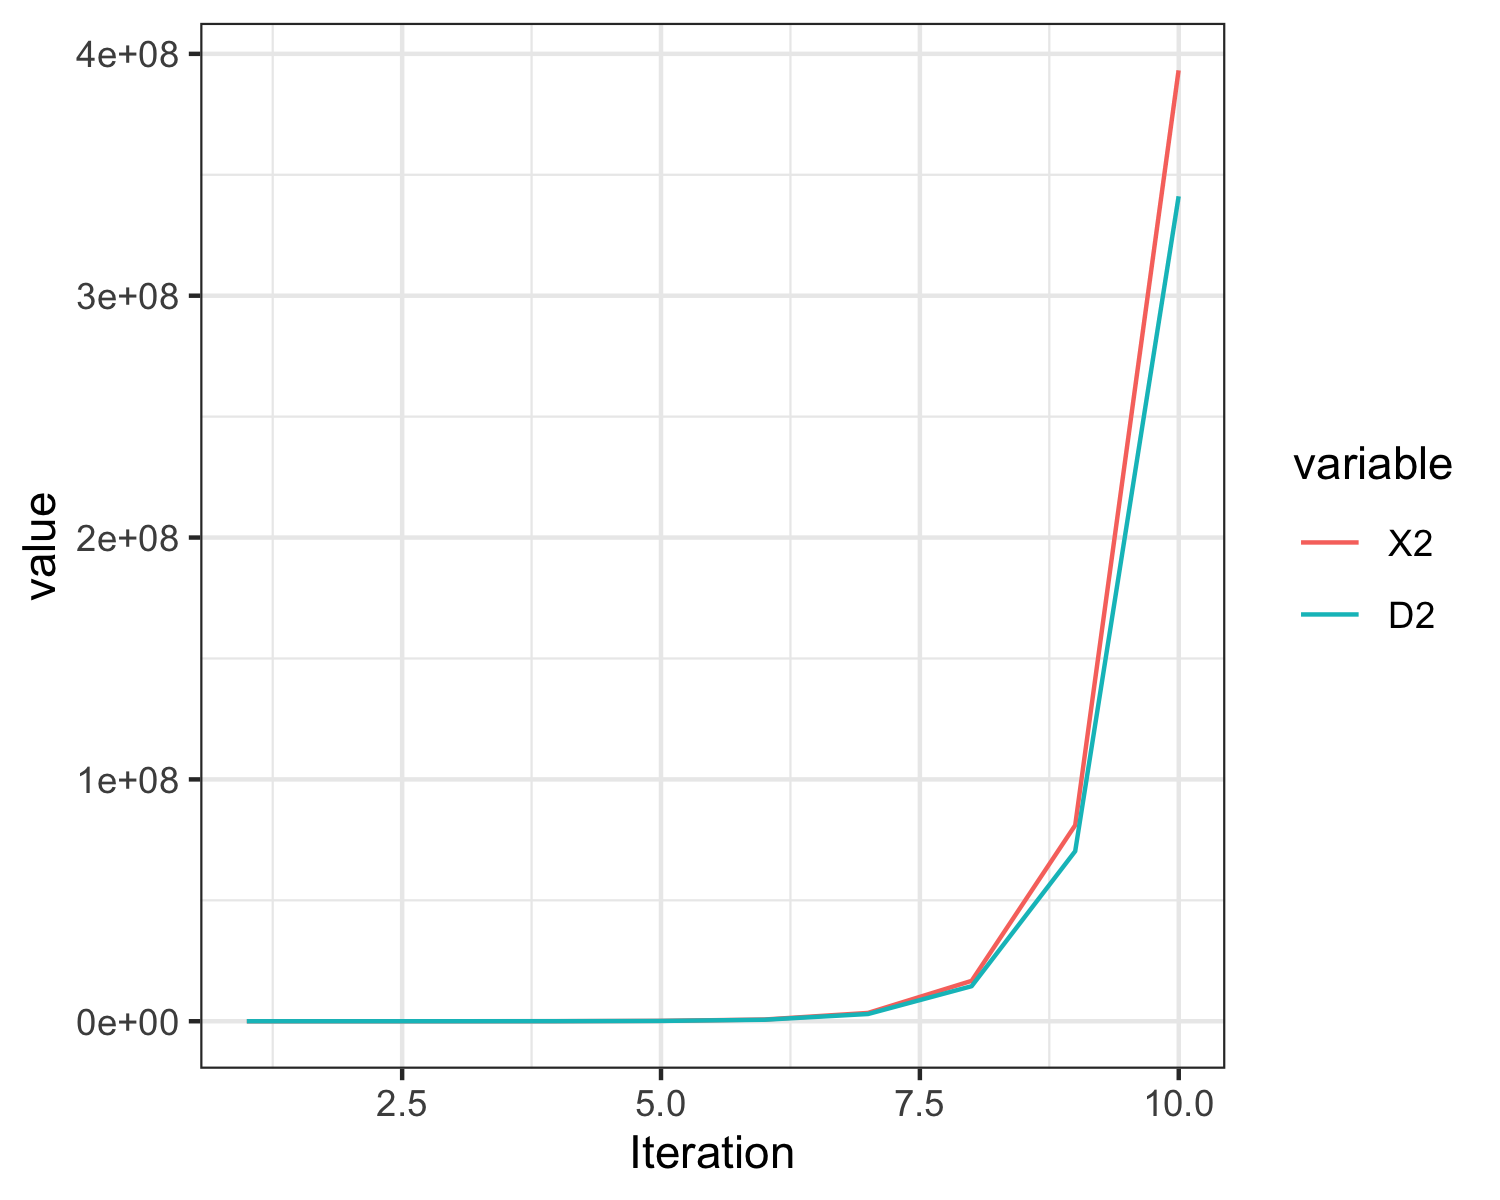
\includegraphics[width=\textwidth]{../../../output/figures/Optimization/x2_plot.png}
          \caption{Mean value of $X_2^i,D_2^i$}

        \end{subfigure}
        \caption{Mean values of $X_1^i,X_2^i,D_1^i,D_2^i$ in each iteration}
        \label{fig-em}
    \end{figure}


\end{document}
